\documentclass{article}
\usepackage{graphicx}

\pagestyle{myheadings}
\title { Some Mastermind Puzzles }
\author{Duncan C. White}

\begin{document}
\maketitle

\renewcommand{\baselinestretch}{0.5}

\section*{What is it}

Remember Mastermind (the board game, not the TV quiz)?  You try to guess
a secret code, using colours (possibly repeated) stuck in some number of
positions, or holes.
In examples shown here, there are 3, 4 or 5 colours chosen from:
Red, Green, Blue, Yellow and Pink, and 3, 4 or 5 positions to fill.

Each go, you make a guess - a sequence of colours, possibly repeated, such
as {\bf RGB}.
This is then scored against the secret code, giving a number of {\bf black pegs} and a number of {\bf white pegs}.

\begin{enumerate}
\item
You are given a {\em black peg} for an exactly correct colour - the
correct colour in the correct place.  Of course, you are not told
which position(s) contain the correct colour, simply how many positions
contain the correct colour.

\item
You are given a {\em white peg} for a misplaced colour - the correct
colour but in a different place.

\end{enumerate}

\par\noindent
So, for example, if the secret code was:


\includegraphics[width=3cm]{secret.png}

\par\noindent
and you guessed:


\includegraphics[width=3cm]{guess.png}

\par\noindent
Then you would score {\bf 1 black peg} for the exactly correct Red in the third
position, and {\bf 1 white peg} for the misplaced Yellow in the second position
(matching the secret code's Yellow in the first position).  This score would be shown as:


\includegraphics[width=1cm]{pegs.png}

\section*{What To Do}

For each example, your task is to find a ``next guess" that is compatible
with all previous guesses and their scores.  There is exactly one such
compatible guess for each (which is of course the secret code):

\begin{tabular}{l l}

{\bf Example 1: 4 colours: R,G,B,Y}    & {\bf Example 2: 4 colours: R,G,B,Y} \\
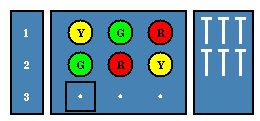
\includegraphics[width=6cm]{eg1.png}   & 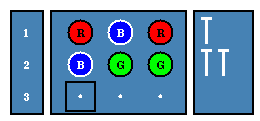
\includegraphics[width=6cm]{eg2.png} \\

{\bf Example 3: 4 colours: R,G,B,Y}    & {\bf Example 4: 4 colours: R,G,B,Y} \\
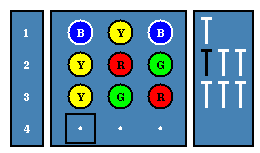
\includegraphics[width=6cm]{eg3.png}   & 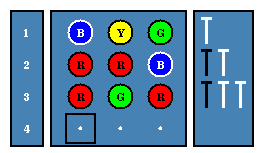
\includegraphics[width=6cm]{eg4.png} \\

{\bf Example 5: 3 colours: R,G,B}     \\
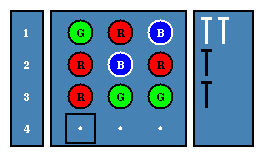
\includegraphics[width=6cm]{eg5.png}  \\

\end{tabular}

\end{document}
